

\subsection{Repeating Things: For-Loops}

Karl's next aim is to add little ticks on the axes at positions $-1$, $-1/2$,
$1/2$, and $1$. For this, it would be nice to use some kind of ``loop'',
especially since he wishes to do the same thing at each of these positions.
There are different packages for doing this. \LaTeX\ has its own internal
command for this, |pstricks| comes along with the powerful |\multido| command.
All of these can be used together with \tikzname, so if you are familiar with
them, feel free to use them. \tikzname\ introduces yet another command, called
|\foreach|, which I introduced since I could never remember the syntax of the
other packages. |\foreach| is defined in the package |pgffor| and can be used
independently of \tikzname, but \tikzname\ includes it automatically.

In its basic form, the |\foreach| command is easy to use:
%
\begin{codeexample}[]
\foreach \x in {1,2,3} {$x =\x$, }
\end{codeexample}

The general syntax is
|\foreach| \meta{variable}| in {|\meta{list of values}|} |\meta{commands}.
Inside the \meta{commands}, the \meta{variable} will be assigned to the
different values. If the \meta{commands} do not start with a brace, everything
up to the next semicolon is used as \meta{commands}.

For Karl and the ticks on the axes, he could use the following code:
%
\begin{codeexample}[]
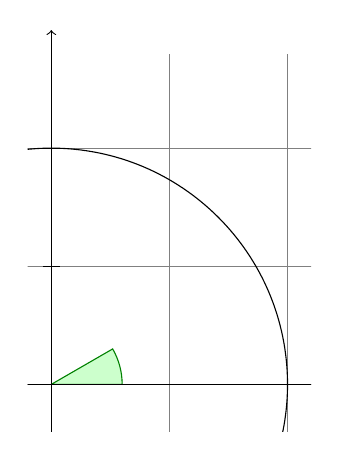
\begin{tikzpicture}[scale=3]
  \clip (-0.1,-0.2) rectangle (1.1,1.51);
  \draw[step=.5cm,gray,very thin] (-1.4,-1.4) grid (1.4,1.4);
  \filldraw[fill=green!20,draw=green!50!black] (0,0) -- (3mm,0mm)
      arc [start angle=0, end angle=30, radius=3mm] -- cycle;
  \draw[->] (-1.5,0) -- (1.5,0);
  \draw[->] (0,-1.5) -- (0,1.5);
  \draw (0,0) circle [radius=1cm];

  \foreach \x in {-1cm,-0.5cm,1cm}
    \draw (\x,-1pt) -- (\x,1pt);
  \foreach \y in {-1cm,-0.5cm,0.5cm,1cm}
    \draw (-1pt,\y) -- (1pt,\y);
\end{tikzpicture}
\end{codeexample}

As a matter of fact, there are many different ways of creating the ticks. For
example, Karl could have put the |\draw ...;| inside curly braces. He could
also have used, say,
%
\begin{codeexample}[code only]
\foreach \x in {-1,-0.5,1}
  \draw[xshift=\x cm] (0pt,-1pt) -- (0pt,1pt);
\end{codeexample}

Karl is curious what would happen in a more complicated situation where there
are, say, 20 ticks. It seems bothersome to explicitly mention all these numbers
in the set for |\foreach|. Indeed, it is possible to use |...| inside the
|\foreach| statement to iterate over a large number of values (which must,
however, be dimensionless real numbers) as in the following example:
%
\begin{codeexample}[]
\tikz \foreach \x in {1,...,10}
        \draw (\x,0) circle (0.4cm);
\end{codeexample}

If you provide \emph{two} numbers before the |...|, the |\foreach| statement
will use their difference for the stepping:
%
\begin{codeexample}[]
\tikz \foreach \x in {-1,-0.5,...,1}
       \draw (\x cm,-1pt) -- (\x cm,1pt);
\end{codeexample}

We can also nest loops to create interesting effects:
%
\begin{codeexample}[]
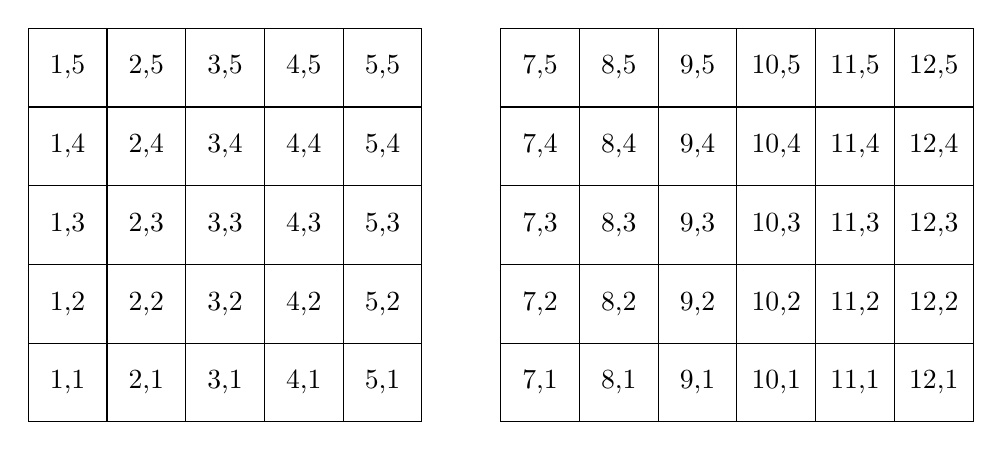
\begin{tikzpicture}
  \foreach \x in {1,2,...,5,7,8,...,12}
    \foreach \y in {1,...,5}
    {
      \draw (\x,\y) +(-.5,-.5) rectangle ++(.5,.5);
      \draw (\x,\y) node{\x,\y};
    }
\end{tikzpicture}
\end{codeexample}

The |\foreach| statement can do even trickier stuff, but the above gives the
idea.

\mshowc{section}
\mshowc{subsection}
\mshowc{subsubsection}
\end{document}

\subsection{Adding Text}

Karl is, by now, quite satisfied with the picture. However, the most important
parts, namely the labels, are still missing!

\tikzname\ offers an easy-to-use and powerful system for adding text and, more
generally, complex shapes to a picture at specific positions. The basic idea is
the following: When \tikzname\ is constructing a path and encounters the
keyword |node| in the middle of a path, it reads a \emph{node specification}.
The keyword |node| is typically followed by some options and then some text
between curly braces. This text is put inside a normal \TeX\ box (if the node
specification directly follows a coordinate, which is usually the case,
\tikzname\ is able to perform some magic so that it is even possible to use
verbatim text inside the boxes) and then placed at the current position, that
is, at the last specified position (possibly shifted a bit, according to the
given options). However, all nodes are drawn only after the path has been
completely drawn/filled/shaded/clipped/whatever.
%
\begin{codeexample}[]
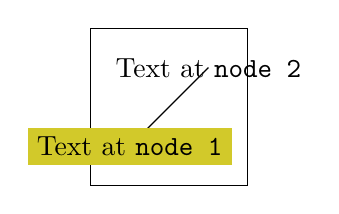
\begin{tikzpicture}
  \draw (0,0) rectangle (2,2);
  \draw (0.5,0.5) node [fill=yellow!80!black]
                       {Text at \verb!node 1!}
     -- (1.5,1.5) node {Text at \verb!node 2!};
\end{tikzpicture}
\end{codeexample}

Obviously, Karl would not only like to place nodes \emph{on} the last specified
position, but also to the left or the right of these positions. For this, every
node object that you put in your picture is equipped with several
\emph{anchors}. For example, the |north| anchor is in the middle at the upper
end of the shape, the |south| anchor is at the bottom and the |north east|
anchor is in the upper right corner. When you give the option |anchor=north|,
the text will be placed such that this northern anchor will lie on the current
position and the text is, thus, below the current position. Karl uses this to
draw the ticks as follows:
%
\begin{codeexample}[]
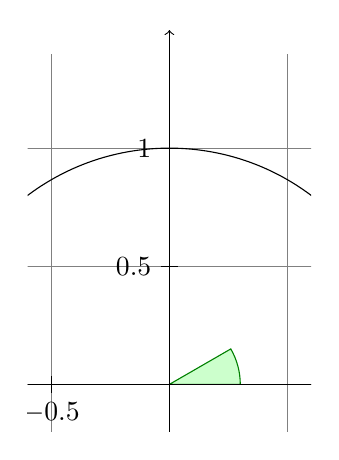
\begin{tikzpicture}[scale=3]
  \clip (-0.6,-0.2) rectangle (0.6,1.51);
  \draw[step=.5cm,help lines] (-1.4,-1.4) grid (1.4,1.4);
  \filldraw[fill=green!20,draw=green!50!black] (0,0) -- (3mm,0mm)
    arc [start angle=0, end angle=30, radius=3mm] -- cycle;
  \draw[->] (-1.5,0) -- (1.5,0);   \draw[->] (0,-1.5) -- (0,1.5);
  \draw (0,0) circle [radius=1cm];

  \foreach \x in {-1,-0.5,1}
    \draw (\x cm,1pt) -- (\x cm,-1pt) node[anchor=north] {$\x$};
  \foreach \y in {-1,-0.5,0.5,1}
    \draw (1pt,\y cm) -- (-1pt,\y cm) node[anchor=east] {$\y$};
\end{tikzpicture}
\end{codeexample}

This is quite nice, already. Using these anchors, Karl can now add most of the
other text elements. However, Karl thinks that, though ``correct'', it is quite
counter-intuitive that in order to place something \emph{below} a given point,
he has to use the \emph{north} anchor. For this reason, there is an option
called |below|, which does the same as |anchor=north|. Similarly, |above right|
does the same as |anchor=south west|. In addition, |below| takes an optional
dimension argument. If given, the shape will additionally be shifted downwards
by the given amount. So, |below=1pt| can be used to put a text label below some
point and, additionally shift it  1pt downwards.

Karl is not quite satisfied with the ticks. He would like to have $1/2$ or
$\frac{1}{2}$ shown instead of $0.5$, partly to show off the nice capabilities
of \TeX\ and \tikzname, partly because for positions like $1/3$ or $\pi$ it is
certainly very much preferable to have the ``mathematical'' tick there instead
of just the ``numeric'' tick. His students, on the other hand, prefer $0.5$
over $1/2$ since they are not too fond of fractions in general.

Karl now faces a problem: For the |\foreach| statement, the position |\x|
should still be given as |0.5| since \tikzname\ will not know where
|\frac{1}{2}| is supposed to be. On the other hand, the typeset text should
really be  |\frac{1}{2}|. To solve this problem, |\foreach| offers a special
syntax: Instead of having one variable |\x|, Karl can specify two (or even
more) variables separated by a slash as in |\x / \xtext|. Then, the elements in
the set over which |\foreach| iterates must also be of the form
\meta{first}|/|\meta{second}. In each iteration, |\x| will be set to
\meta{first} and |\xtext| will be set to \meta{second}. If no \meta{second} is
given, the \meta{first} will be used again. So, here is the new code for the
ticks:
%
\begin{codeexample}[]
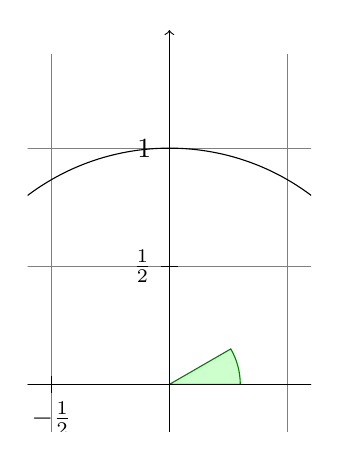
\begin{tikzpicture}[scale=3]
  \clip (-0.6,-0.2) rectangle (0.6,1.51);
  \draw[step=.5cm,help lines] (-1.4,-1.4) grid (1.4,1.4);
  \filldraw[fill=green!20,draw=green!50!black] (0,0) -- (3mm,0mm)
      arc [start angle=0, end angle=30, radius=3mm] -- cycle;
  \draw[->] (-1.5,0) -- (1.5,0); \draw[->] (0,-1.5) -- (0,1.5);
  \draw (0,0) circle [radius=1cm];

  \foreach \x/\xtext in {-1, -0.5/-\frac{1}{2}, 1}
    \draw (\x cm,1pt) -- (\x cm,-1pt) node[anchor=north] {$\xtext$};
  \foreach \y/\ytext in {-1, -0.5/-\frac{1}{2}, 0.5/\frac{1}{2}, 1}
    \draw (1pt,\y cm) -- (-1pt,\y cm) node[anchor=east] {$\ytext$};
\end{tikzpicture}
\end{codeexample}

Karl is quite pleased with the result, but his son points out that this is
still not perfectly satisfactory: The grid and the circle interfere with the
numbers and decrease their legibility. Karl is not very concerned by this (his
students do not even notice), but his son insists that there is an easy
solution: Karl can add the |[fill=white]| option to fill out the background of
the text shape with a white color.

The next thing Karl wants to do is to add the labels like $\sin \alpha$. For
this, he would like to place a label ``in the middle of the line''. To do so,
instead of specifying the label |node {$\sin\alpha$}|  directly after one of
the endpoints of the line (which would place the label at that endpoint), Karl
can give the label directly after the |--|, before the coordinate. By default,
this places the label in the middle of the line, but the |pos=| options can be
used to modify this. Also, options like |near start| and |near end| can be used
to modify this position:
%
\begin{codeexample}[preamble={\usetikzlibrary{intersections}}]
\begin{tikzpicture}[scale=3]
  \clip (-2,-0.2) rectangle (2,0.8);
  \draw[step=.5cm,gray,very thin] (-1.4,-1.4) grid (1.4,1.4);
  \filldraw[fill=green!20,draw=green!50!black] (0,0) -- (3mm,0mm)
    arc [start angle=0, end angle=30, radius=3mm] -- cycle;
  \draw[->] (-1.5,0) -- (1.5,0) coordinate (x axis);
  \draw[->] (0,-1.5) -- (0,1.5) coordinate (y axis);
  \draw (0,0) circle [radius=1cm];

  \draw[very thick,red]
    (30:1cm) -- node[left=1pt,fill=white] {$\sin \alpha$} (30:1cm |- x axis);
  \draw[very thick,blue]
    (30:1cm |- x axis) -- node[below=2pt,fill=white] {$\cos \alpha$} (0,0);
  \path [name path=upward line] (1,0) -- (1,1);
  \path [name path=sloped line] (0,0) -- (30:1.5cm);
  \draw [name intersections={of=upward line and sloped line, by=t}]
    [very thick,orange] (1,0) -- node [right=1pt,fill=white]
    {$\displaystyle \tan \alpha \color{black}=
      \frac{{\color{red}\sin \alpha}}{\color{blue}\cos \alpha}$} (t);

  \draw (0,0) -- (t);

  \foreach \x/\xtext in {-1, -0.5/-\frac{1}{2}, 1}
    \draw (\x cm,1pt) -- (\x cm,-1pt) node[anchor=north,fill=white] {$\xtext$};
  \foreach \y/\ytext in {-1, -0.5/-\frac{1}{2}, 0.5/\frac{1}{2}, 1}
    \draw (1pt,\y cm) -- (-1pt,\y cm) node[anchor=east,fill=white] {$\ytext$};
\end{tikzpicture}
\end{codeexample}

You can also position labels on curves and, by adding the |sloped| option, have
them rotated such that they match the line's slope. Here is an example:
%
\begin{codeexample}[]
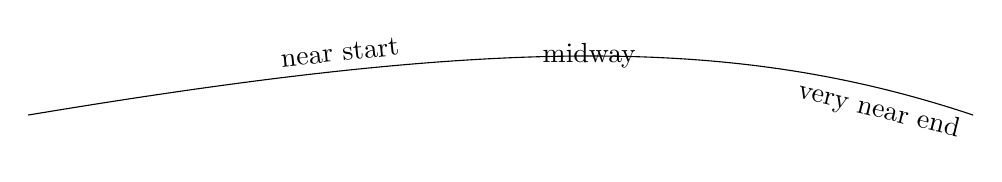
\begin{tikzpicture}
  \draw (0,0) .. controls (6,1) and (9,1) ..
    node[near start,sloped,above] {near start}
    node {midway}
    node[very near end,sloped,below] {very near end} (12,0);
\end{tikzpicture}
\end{codeexample}

It remains to draw the explanatory text at the right of the picture. The main
difficulty here lies in limiting the width of the text ``label'', which is
quite long, so that line breaking is used. Fortunately, Karl can use the option
|text width=6cm| to get the desired effect. So, here is the full code:
%
\begin{codeexample}[code only]
\begin{tikzpicture}
  [scale=3,line cap=round,
  % Styles
  axes/.style=,
  important line/.style={very thick},
  information text/.style={rounded corners,fill=red!10,inner sep=1ex}]

  % Colors
  \colorlet{anglecolor}{green!50!black}
  \colorlet{sincolor}{red}
  \colorlet{tancolor}{orange!80!black}
  \colorlet{coscolor}{blue}

  % The graphic
  \draw[help lines,step=0.5cm] (-1.4,-1.4) grid (1.4,1.4);

  \draw (0,0) circle [radius=1cm];

  \begin{scope}[axes]
    \draw[->] (-1.5,0) -- (1.5,0) node[right] {$x$} coordinate(x axis);
    \draw[->] (0,-1.5) -- (0,1.5) node[above] {$y$} coordinate(y axis);

    \foreach \x/\xtext in {-1, -.5/-\frac{1}{2}, 1}
      \draw[xshift=\x cm] (0pt,1pt) -- (0pt,-1pt) node[below,fill=white] {$\xtext$};

    \foreach \y/\ytext in {-1, -.5/-\frac{1}{2}, .5/\frac{1}{2}, 1}
      \draw[yshift=\y cm] (1pt,0pt) -- (-1pt,0pt) node[left,fill=white] {$\ytext$};
  \end{scope}

  \filldraw[fill=green!20,draw=anglecolor] (0,0) -- (3mm,0pt)
    arc [start angle=0, end angle=30, radius=3mm];
  \draw (15:2mm) node[anglecolor] {$\alpha$};

  \draw[important line,sincolor]
    (30:1cm) -- node[left=1pt,fill=white] {$\sin \alpha$} (30:1cm |- x axis);

  \draw[important line,coscolor]
    (30:1cm |- x axis) -- node[below=2pt,fill=white] {$\cos \alpha$} (0,0);

  \path [name path=upward line] (1,0) -- (1,1);
  \path [name path=sloped line] (0,0) -- (30:1.5cm);
  \draw [name intersections={of=upward line and sloped line, by=t}]
    [very thick,orange] (1,0) -- node [right=1pt,fill=white]
    {$\displaystyle \tan \alpha \color{black}=
      \frac{{\color{red}\sin \alpha}}{\color{blue}\cos \alpha}$} (t);

  \draw (0,0) -- (t);

  \draw[xshift=1.85cm]
    node[right,text width=6cm,information text]
    {
      The {\color{anglecolor} angle $\alpha$} is $30^\circ$ in the
      example ($\pi/6$ in radians). The {\color{sincolor}sine of
        $\alpha$}, which is the height of the red line, is
      \[
      {\color{sincolor} \sin \alpha} = 1/2.
      \]
      By the Theorem of Pythagoras ...
    };
\end{tikzpicture}
\end{codeexample}


\subsection{Pics: The Angle Revisited}

Karl expects that the code of certain parts of the picture he created might be
so useful that he might wish to reuse them in the future. A natural thing to do
is to create \TeX\ macros that store the code he wishes to reuse. However,
\tikzname\ offers another way that is integrated directly into its parser:
pics!

A ``pic'' is ``not quite a full picture'', hence the short name. The idea is
that a pic is simply some code that you can add to a picture at different
places using the |pic| command whose syntax is almost identical to the |node|
command. The main difference is that instead of specifying some text in curly
braces that should be shown, you specify the name of a predefined picture that
should be shown.

Defining new pics is easy enough, see Section~\ref{section-pics}, but right now
we just want to use one such predefined pic: the |angle| pic. As the name
suggests, it is a small drawing of an angle consisting of a little wedge and an
arc together with some text (Karl needs to load the |angles| library and the
|quotes| for the following examples). What makes this pic useful is the fact
that the size of the wedge will be computed automatically.

The |angle| pic draws an angle between the two lines $BA$ and $BC$, where $A$,
$B$, and $C$ are three coordinates. In our case, $B$ is the origin, $A$ is
somewhere on the $x$-axis and $C$ is somewhere on a line at $30^\circ$.
%
\begin{codeexample}[preamble={\usetikzlibrary{angles,quotes}}]
\begin{tikzpicture}[scale=3]
  \coordinate (A) at (1,0);
  \coordinate (B) at (0,0);
  \coordinate (C) at (30:1cm);

  \draw (A) -- (B) -- (C)
        pic [draw=green!50!black, fill=green!20, angle radius=9mm,
             "$\alpha$"] {angle = A--B--C};
\end{tikzpicture}
\end{codeexample}

Let us see, what is happening here. First we have specified three
\emph{coordinates} using the |\coordinate| command. It allows us to name a
specific coordinate in the picture. Then comes something that starts as a
normal |\draw|, but then comes the |pic| command. This command gets lots of
options and, in curly braces, comes the most important point: We specify that
we want to add an |angle| pic and this angle should be between the points we
named |A|, |B|, and |C| (we could use other names). Note that the text that we
want to be shown in the pic is specified in quotes inside the options of the
|pic|, not inside the curly braces.

To learn more about pics, please see Section~\ref{section-pics}.
